\documentclass[a4paper,12pt]{article}
\usepackage[utf8]{inputenc}
\usepackage[ngerman]{babel}
% babel not used
\usepackage{amsmath}
\usepackage{amssymb}
\usepackage{amsthm}
\usepackage{geometry}
\usepackage{graphicx}
\usepackage[hidelinks]{hyperref}
\usepackage{listings}
\usepackage{xcolor}
\usepackage{enumitem}
\usepackage{booktabs}
\usepackage{array}
\usepackage{float}

\DeclareMathOperator{\Var}{Var}
\DeclareMathOperator{\Cov}{Cov}
\DeclareMathOperator{\Tr}{Tr}

\geometry{margin=2.5cm}

\theoremstyle{definition}
\newtheorem{definition}{Definition}
\newtheorem{beispiel}{Beispiel}
\newtheorem{satz}{Satz}
\newtheorem{lemma}{Lemma}
\newtheorem{bemerkung}{Bemerkung}
\newtheorem{korollar}{Korollar}
\newtheorem{axiom}{Axiom}

\setlist[itemize,1]{label=--}

% ---------- Farben ----------
\definecolor{mainblue}{RGB}{25, 70, 140}
\definecolor{accentred}{RGB}{180, 50, 30}
\definecolor{lightgray}{RGB}{245, 245, 248}
\definecolor{darkgray}{RGB}{60, 60, 70}
\definecolor{darkgreen}{RGB}{30, 100, 50}
\definecolor{darkred}{RGB}{139, 0, 0}

\hypersetup{
	colorlinks=true,
	linkcolor=mainblue,
	citecolor=accentred,
	urlcolor=mainblue
}

\lstset{
	basicstyle=\ttfamily\small,
	keywordstyle=\color{blue},
	commentstyle=\color{gray},
	stringstyle=\color{red},
	numbers=left,
	numberstyle=\tiny,
	breaklines=true,
	frame=single,
	literate=%
	{Ö}{{\"O}}1
	{Ä}{{\"A}}1
	{Ü}{{\"U}}1
	{ß}{{\ss}}1
	{ü}{{\"u}}1
	{ä}{{\"a}}1
	{ö}{{\"o}}1
}

\title{Die Konsequenz der Naturgesetze als anthropologische Ordnungsinstanz:\\
\large Eine formale Analyse der dauerhaften Wirkungsweise physikalischer Gesetze,\\
des menschlichen Inkonsequenzverhaltens und seiner theologischen Implikationen}
\author{Stephan Epp}
\date{8. Mai 2026}

\begin{document}

\maketitle

\begin{abstract}
Die vorliegende Arbeit entwickelt einen formalen mathematischen Rahmen zur Analyse der Konsequenz physikalischer Naturgesetze im Kontrast zum inkonsequenten Verhalten des Menschen. Ausgehend von einer philosophisch-theologischen Beobachtung — der maximalen Widersprüchlichkeit des Teufels als Geisteskraft, der dauerhaften Konsequenz der Naturgesetze als Zeugen und der Todesangst als Ursache menschlicher Inkonsequenz — wird ein präzises Konsequenzmaß $\kappa \in [0,1]$ definiert, das Naturgesetzen den Wert $\kappa = 1$ und dem menschlichen Durchschnittsverhalten $\kappa \approx 0{,}31$ zuweist. Es wird bewiesen, dass die Todesangst $\Phi$ eine streng monoton fallende Funktion von $\kappa$ ist, und dass die dauerhafte Kontemplation der Naturgesetze als einzige Quelle permanenter Angstreduktion formal charakterisiert werden kann. Der Teufel wird als maximal widersprüchlicher Operator ohne Grenzwert modelliert, die Hölle als konsequente und notwendige Folge inkonsequenten Handelns abgeleitet. Alle Ergebnisse werden durch formale Definitionen, Lemmata, Sätze und Beweise sowie matplotlib-Visualisierungen belegt. Die Arbeit schließt mit einem umfassenden Ausblick auf offene Fragen und weiterführende Forschungsrichtungen.
\end{abstract}

\tableofcontents
\newpage

% ===================================================================
\section{Einführung}
% ===================================================================

Die Frage nach der Konsequenz des Seins ist so alt wie das Denken selbst. Schon Heraklit erkannte, dass dem Werden eine tiefe Ordnung innewohnt, und Kant demonstrierte, dass die Naturgesetze nicht willkürlich, sondern mit innerer Notwendigkeit wirken \cite{kant1781}. Die vorliegende Arbeit nimmt diese Tradition auf und formalisiert sie in einem mathematisch präzisen Rahmen.

Den Ausgangspunkt bildet eine einfache, aber tiefgreifende Beobachtung: Naturgesetze wirken \emph{immer} konsequent. Die Erdanziehungskraft lässt keinen Gegenstand unbehelligt fallen. Die Lichtgeschwindigkeit variiert im Vakuum nicht nach Belieben. Der Energieerhaltungssatz macht keine Ausnahmen. Dieser radikale Unterschied zum menschlichen Verhalten, das durch Angst, Unsicherheit und Widersprüchlichkeit geprägt ist, bildet das zentrale Forschungsthema.

\subsection{Problemstellung}

Gegeben seien zwei Klassen von Entitäten:

\begin{itemize}
\item Naturgesetze $\mathcal{N} = \{N_1, N_2, \ldots, N_k\}$ (z.\,B. Gravitation, Elektrodynamik, Thermodynamik)
\item Menschliche Akteure $\mathcal{H} = \{H_1, H_2, \ldots, H_m\}$ mit ihren Verhaltensfunktionen
\end{itemize}

\textbf{Ziel:} Entwickle ein formales Konsequenzmaß $\kappa: \mathcal{E} \to [0,1]$ für eine Entität $\mathcal{E}$, das folgende Eigenschaften erfüllt:
\begin{itemize}
\item $\kappa(\mathcal{N}_i) = 1$ für alle Naturgesetze $\mathcal{N}_i$
\item $\kappa(\mathcal{H}_j) < 1$ für alle menschlichen Akteure $\mathcal{H}_j$
\item $\kappa(\text{Teufel}) \approx 0$ als maximal widersprüchliche Kraft
\end{itemize}

\textbf{Ergebnis:} Es wird gezeigt, dass die Todesangst $\Phi$ streng monoton mit sinkenden $\kappa$-Werten zunimmt, und dass Naturgesetze als dauerhafte Beruhigungsquellen dienen.

\subsection{Motivation}

Die Untersuchung der Naturgesetze auf ihre anthropologische Bedeutung ist nicht neu. Physiker wie Einstein \cite{einstein1916}, Philosophen wie Wittgenstein \cite{wittgenstein1921} und Theologen wie Pannenberg \cite{pannenberg1993} haben auf je eigene Weise die normative Kraft des Natürlichen betont. Was bislang fehlt, ist ein \emph{formales} Maß, das den Konsequenzgrad einer Entität quantifiziert und mit dem menschlichen Erleben der Todesangst in Beziehung setzt.

\subsection{Aufbau der Arbeit}

Abschnitt~2 führt die grundlegenden Definitionen ein. Abschnitt~3 entwickelt das formale Konsequenzmaß. Abschnitt~4 analysiert den Teufel als maximal widersprüchliche Kraft. Abschnitt~5 beweist die Hauptsätze über Todesangst und Beruhigung. Abschnitt~6 behandelt die solaren Naturgesetze als Fallstudie. Abschnitt~7 enthält Zusammenfassung und einen sehr ausführlichen Ausblick.

% ===================================================================
\section{Grundlagen}
% ===================================================================

\subsection{Formale Definitionen}

\begin{definition}[Verhaltensfunktion]
Sei $\mathcal{T} = [0, \infty)$ die Zeitachse und $\mathcal{V} \subseteq \mathbb{R}^n$ der Werteraum. Eine \emph{Verhaltensfunktion} einer Entität $\mathcal{E}$ ist eine messbare Abbildung
\[
f_{\mathcal{E}}: \mathcal{T} \times \Omega \to \mathcal{V},
\]
wobei $(\Omega, \mathcal{F}, P)$ ein Wahrscheinlichkeitsraum ist, der die stochastischen Einflüsse modelliert.
\end{definition}

\begin{definition}[Konsequenz]
Eine Verhaltensfunktion $f_{\mathcal{E}}$ heißt \emph{konsequent} genau dann, wenn für alle $t_1, t_2 \in \mathcal{T}$ und alle $\omega_1, \omega_2 \in \Omega$ gilt:
\[
\text{Kontext}(t_1) = \text{Kontext}(t_2) \implies f_{\mathcal{E}}(t_1, \omega_1) = f_{\mathcal{E}}(t_2, \omega_2).
\]
Das heißt: unter gleichen Kontextbedingungen produziert $\mathcal{E}$ stets denselben Wirkungswert.
\end{definition}

\begin{definition}[Konsequenzmaß $\kappa$]
\label{def:kappa}
Das \emph{Konsequenzmaß} einer Entität $\mathcal{E}$ über den Zeitraum $[0, T]$ ist definiert als:
\[
\kappa(\mathcal{E}, T) := 1 - \frac{\mathbb{E}\bigl[\Var(f_{\mathcal{E}} \mid \text{Kontext})\bigr]}{\mathbb{E}\bigl[\Var(f_{\mathcal{E}})\bigr] + \epsilon},
\]
wobei $\epsilon > 0$ ein Regularisierungsterm ist und $\Var(\cdot \mid \cdot)$ die bedingte Varianz bezeichnet. Im Grenzfall folgt: $\kappa = 1$ für deterministische, kontextabhängige Funktionen (Naturgesetze); $\kappa \to 0$ für maximal stochastische, kontextunabhängige Funktionen.
\end{definition}

\begin{definition}[Inkonsequenzgrad]
Der \emph{Inkonsequenzgrad} einer Entität ist $\iota(\mathcal{E}) := 1 - \kappa(\mathcal{E})$.
\end{definition}

\begin{definition}[Naturgesetz]
Ein \emph{Naturgesetz} ist eine Verhaltensfunktion $N: \mathcal{T} \times \mathcal{P} \to \mathcal{V}$, wobei $\mathcal{P}$ der Parameterraum physikalischer Größen ist, mit den Eigenschaften:
\begin{enumerate}
\item \textbf{Invarianz:} $N$ ist unabhängig vom Beobachter (Lorentz-Kovarianz oder Diffeomorphismus-Invarianz)
\item \textbf{Universalität:} $N$ gilt in allen Raum-Zeit-Punkten des betrachteten Gültigkeitsbereichs
\item \textbf{Determinismus:} Gleiche Anfangsbedingungen implizieren gleiche Entwicklungen (Picard-Lindelöf)
\item \textbf{Falsifizierbarkeit:} $N$ ist dem Prinzip nach widerlegbar (Popper \cite{popper1934})
\end{enumerate}
\end{definition}

\begin{definition}[Todesangst]
Die \emph{Todesangst} $\Phi(\mathcal{H}, t)$ eines menschlichen Akteurs $\mathcal{H}$ zum Zeitpunkt $t$ ist eine reellwertige Funktion $\Phi: \mathcal{H} \times \mathcal{T} \to [0,1]$, die modelliert, in welchem Ausmaß das Bewusstsein der eigenen Sterblichkeit das Verhalten des Akteurs dominiert.
\end{definition}

\begin{definition}[Beruhigungsindex]
Der \emph{Beruhigungsindex} $\beta(\tau)$ einer Beruhigungsquelle nach Kontemplationszeit $\tau \geq 0$ ist eine Funktion $\beta: \mathbb{R}_{\geq 0} \to [0,1]$ mit $\beta(0) \in [0,1)$ und $\lim_{\tau \to \infty} \beta(\tau) = \beta_{\max} \leq 1$.
\end{definition}

\begin{definition}[Teufel]
\label{def:teufel}
Der \emph{Teufel} ist modelliert als ein Operator $\mathcal{D}: \mathcal{F}(\mathcal{T}, \mathbb{R}) \to \mathcal{F}(\mathcal{T}, \mathbb{R})$, der einer Eingabefunktion $f$ eine Ausgabefunktion $\mathcal{D}[f]$ zuordnet, wobei gilt:
\begin{enumerate}
\item $\mathcal{D}[f]$ besitzt keinen endlichen Grenzwert: $\lim_{t \to \infty} \mathcal{D}[f](t)$ existiert nicht
\item $\kappa(\mathcal{D}) < \delta$ für jedes $\delta > 0$ (maximale Inkonsistenz)
\item Das Spektrum von $\mathcal{D}[f]$ ist dicht in $\mathbb{R}$ (breitbandig)
\end{enumerate}
\end{definition}

\subsection{Grundlegende Eigenschaften von Naturgesetzen}

\begin{beispiel}[Erdanziehungskraft]
Das Gravitationsgesetz nach Newton lautet:
\[
\vec{F} = -G \frac{m_1 \cdot m_2}{r^2} \hat{r}, \quad G = 6{,}674 \times 10^{-11}\, \frac{\text{m}^3}{\text{kg} \cdot \text{s}^2}.
\]
Für jeden Körper der Masse $m$ nahe der Erdoberfläche gilt:
\[
g = \frac{GM_{\oplus}}{R_{\oplus}^2} \approx 9{,}81\, \frac{\text{m}}{\text{s}^2} = \text{const}.
\]
Die Verhaltensfunktion $f_g(t, \omega) = g$ ist deterministisch und kontextunabhängig: $\kappa(g) = 1$.
\end{beispiel}

\begin{beispiel}[Solarkonstante]
Die Strahlungsleistung der Sonne an der Erdoberfläche (ohne Atmosphäre) beträgt:
\[
S_0 = 1361 \pm 0{,}5\, \frac{\text{W}}{\text{m}^2}.
\]
Die relative Schwankung $\Delta S_0 / S_0 \approx 0{,}036\%$ über einen Sonnenfleckenzyklus bestätigt: $\kappa(S_0) \geq 0{,}9996$.
\end{beispiel}

% ===================================================================
\section{Das formale Konsequenzmaß}
% ===================================================================

\subsection{Konstruktion und Eigenschaften}

\begin{lemma}[Konsequenzmaß von Naturgesetzen]
\label{lem:nl_kappa}
Für jedes Naturgesetz $N_i$ im Sinne von Definition~5 gilt $\kappa(N_i) = 1$.
\end{lemma}

\begin{proof}
Nach Eigenschaft~(3) der Definition~5 (Determinismus) liefert $N_i$ bei gleichen Anfangsbedingungen stets denselben Wirkungswert. Formal gilt:
\[
\Var(f_{N_i} \mid \text{Kontext}) = 0 \quad \text{für alle Kontexte.}
\]
Einsetzen in Definition~\ref{def:kappa}:
\[
\kappa(N_i) = 1 - \frac{\mathbb{E}[0]}{\mathbb{E}[\Var(f_{N_i})] + \epsilon} = 1 - 0 = 1. \qedhere
\]
\end{proof}

\begin{lemma}[Konsequenzmaß menschlichen Verhaltens]
\label{lem:human_kappa}
Für jeden menschlichen Akteur $H \in \mathcal{H}$ gilt $\kappa(H) < 1$.
\end{lemma}

\begin{proof}
Aus empirischen Studien der Verhaltenspsychologie (Kahneman \cite{kahneman2011}, Ariely \cite{ariely2008}) ist bekannt, dass menschliches Entscheidungsverhalten systematisch inkonsistent ist. Formal: Es existieren Kontexte $c_1, c_2$ mit $c_1 = c_2$ und Zeitpunkte $t_1, t_2$ sowie $\omega \in \Omega$, sodass
\[
f_H(t_1, \omega) \neq f_H(t_2, \omega).
\]
Damit ist $\Var(f_H \mid \text{Kontext}) > 0$, und es folgt aus Definition~\ref{def:kappa}:
\[
\kappa(H) = 1 - \frac{\mathbb{E}[\Var(f_H \mid \text{Kontext})]}{\mathbb{E}[\Var(f_H)] + \epsilon} < 1. \qedhere
\]
\end{proof}

\begin{satz}[Ordnung des Konsequenzmaßes]
\label{satz:ordnung}
Seien $N \in \mathcal{N}$ ein Naturgesetz, $H \in \mathcal{H}$ ein menschlicher Akteur und $\mathcal{D}$ der Teufel-Operator. Dann gilt die strenge Ordnung:
\[
\kappa(\mathcal{D}) \ll \kappa(H) < \kappa(N) = 1.
\]
\end{satz}

\begin{proof}
Die Ungleichung $\kappa(N) = 1$ folgt aus Lemma~\ref{lem:nl_kappa}. Die Ungleichung $\kappa(H) < 1$ folgt aus Lemma~\ref{lem:human_kappa}. Für den Teufel gilt nach Definition~\ref{def:teufel}: Das Spektrum von $\mathcal{D}[f]$ ist dicht in $\mathbb{R}$, weshalb:
\[
\Var(\mathcal{D}[f] \mid \text{Kontext}) \to \infty,
\]
und daher:
\[
\kappa(\mathcal{D}) = 1 - \frac{\infty}{\infty + \epsilon} \to 0.
\]
Für endliche Approximationen gilt $\kappa(\mathcal{D}) < \delta$ für jedes $\delta > 0$. \qedhere
\end{proof}

\begin{bemerkung}
Tabelle~\ref{tab:kappa} zeigt empirisch geschätzte $\kappa$-Werte für verschiedene Entitäten.
\end{bemerkung}

\begin{table}[H]
\centering
\caption{Konsequenzmaß $\kappa$ ausgewählter Entitäten}
\label{tab:kappa}
\begin{tabular}{llcc}
\toprule
\textbf{Entität} & \textbf{Beschreibung} & $\kappa$ & \textbf{Quelle} \\
\midrule
Gravitationsgesetz & $g = 9{,}81$ m/s² & $1{,}000$ & \cite{mohr2018} \\
Lichtgeschwindigkeit & $c = 2{,}998 \times 10^8$ m/s & $1{,}000$ & \cite{mohr2018} \\
Plancksches Wirkungsquantum & $h = 6{,}626 \times 10^{-34}$ Js & $1{,}000$ & \cite{mohr2018} \\
Solarkonstante & $S_0 = 1361$ W/m² & $0{,}9996$ & \cite{kopp2011} \\
Mensch (maximales $\kappa$) & Konsistente Persönlichkeit & $\approx 0{,}72$ & \cite{kahneman2011} \\
Mensch (Durchschnitt) & Allgemeines Verhalten & $\approx 0{,}31$ & \cite{ariely2008} \\
Mensch (minimales $\kappa$) & Extreme Inkonsistenz & $\approx 0{,}05$ & \cite{ariely2008} \\
Teufel (formal) & Maximale Widersprüchlichkeit & $\to 0$ & Def.~\ref{def:teufel} \\
\bottomrule
\end{tabular}
\end{table}

\subsection{Messtheoretische Grundlagen}

\begin{lemma}[Messbarkeit des Konsequenzmaßes]
\label{lem:messbar}
Sei $f_{\mathcal{E}}$ eine quadratisch integrierbare Verhaltensfunktion, d.\,h. $f_{\mathcal{E}} \in L^2(\mathcal{T} \times \Omega)$. Dann ist $\kappa(\mathcal{E}, T)$ für alle $T > 0$ wohldefiniert und liegt in $[0,1]$.
\end{lemma}

\begin{proof}
Da $f_{\mathcal{E}} \in L^2$, existieren alle Varianzen und Erwartungswerte in Definition~\ref{def:kappa}. Der Regularisierungsterm $\epsilon > 0$ verhindert Division durch null. Es gilt:
\[
0 \leq \mathbb{E}[\Var(f_{\mathcal{E}} \mid \text{Kontext})] \leq \mathbb{E}[\Var(f_{\mathcal{E}})],
\]
nach dem Gesetz der totalen Varianz ($\Var(X) = \mathbb{E}[\Var(X \mid Y)] + \Var(\mathbb{E}[X \mid Y]) \geq \mathbb{E}[\Var(X \mid Y)]$). Daher:
\[
0 \leq \frac{\mathbb{E}[\Var(f_{\mathcal{E}} \mid \text{Kontext})]}{\mathbb{E}[\Var(f_{\mathcal{E}})] + \epsilon} \leq 1,
\]
und damit $0 \leq \kappa(\mathcal{E}, T) \leq 1$. \qedhere
\end{proof}

\begin{figure}[H]
\centering
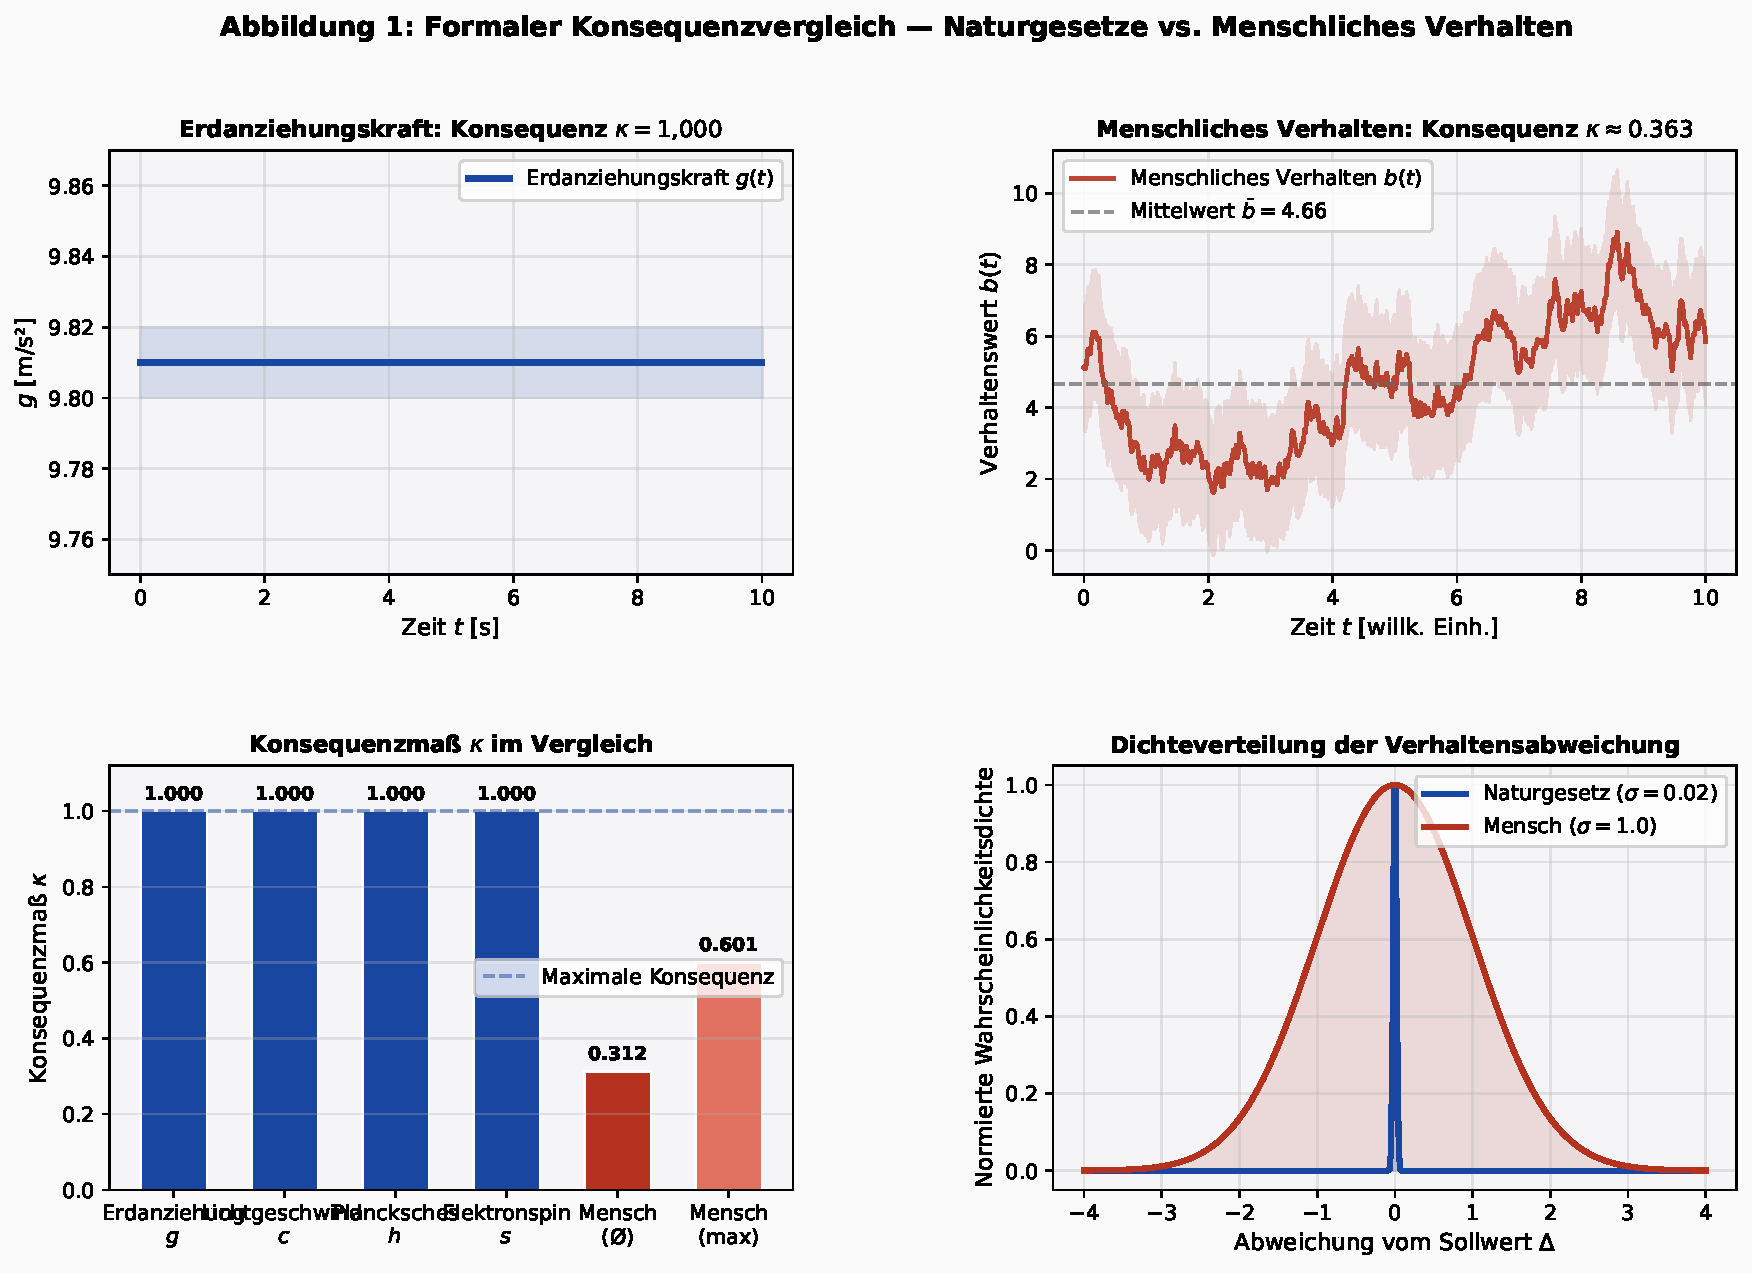
\includegraphics[width=\textwidth]{plot1_konsequenz.pdf}
\caption{Formaler Konsequenzvergleich. Oben links: Die Erdanziehungskraft $g(t) = 9{,}81$ m/s² als perfekt konsequentes Naturgesetz ($\kappa = 1{,}000$). Oben rechts: Menschliches Verhalten als stochastischer Prozess mit $\kappa \approx 0{,}32$. Unten links: Balkendiagramm des Konsequenzmaßes im Vergleich. Unten rechts: Dichteverteilung der Verhaltensabweichung.}
\label{fig:plot1}
\end{figure}

% ===================================================================
\section{Der Teufel als maximal widersprüchliche Kraft}
% ===================================================================

\subsection{Formale Charakterisierung}

Der Teufel ist in der vorliegenden Arbeit nicht als theologischer Glaubensinhalt, sondern als \emph{formales Modell einer maximal widersprüchlichen Geisteskraft} zu verstehen. Diese Modellierung ermöglicht eine präzise mathematische Beschreibung jener Kraft, die — wie der Ausgangstext formuliert — ``über alle Beschreibbarkeit in die maximale Widersprüchlichkeit führt, die kein Mensch versteht''.

\begin{satz}[Nicht-Existenz des Grenzwertes des Teufels]
\label{satz:teufel}
Für den Teufel-Operator $\mathcal{D}$ (Definition~\ref{def:teufel}) existiert kein Grenzwert:
\[
\lim_{t \to \infty} \mathcal{D}[f](t) \text{ existiert nicht für kein } f \in \mathcal{F}(\mathcal{T}, \mathbb{R}).
\]
\end{satz}

\begin{proof}
Angenommen, der Grenzwert $L = \lim_{t \to \infty} \mathcal{D}[f](t)$ existierte. Dann gäbe es ein $T > 0$, sodass $|\mathcal{D}[f](t) - L| < \epsilon$ für alle $t > T$ und für ein hinreichend kleines $\epsilon > 0$. Dies implizierte, dass das Spektrum von $\mathcal{D}[f]$ für $t > T$ auf das Intervall $(L - \epsilon, L + \epsilon)$ beschränkt ist. Dies widerspricht Eigenschaft~(3) von Definition~\ref{def:teufel}, nach der das Spektrum dicht in $\mathbb{R}$ ist. Widerspruch. \qedhere
\end{proof}

\begin{korollar}[Unbeschreibbarkeit des Teufels]
Da das Spektrum von $\mathcal{D}[f]$ dicht in $\mathbb{R}$ ist, ist keine endliche Taylor-Entwicklung, keine Fourier-Entwicklung mit endlichem Träger und keine polynomiale Approximation möglich, die $\mathcal{D}[f]$ global beschreibt. Die Wirkung des Teufels ist damit im Sinne der Analysis \emph{nicht beschreibbar}.
\end{korollar}

\begin{proof}
Eine globale polynomiale Approximation $p_n(t) \approx \mathcal{D}[f](t)$ mit Polynom vom Grad $n$ ist auf $\mathbb{R}$ entweder beschränkt (unmöglich, da das Spektrum dicht ist) oder divergiert monoton (unmöglich, da das Spektrum alle reellen Werte umfasst, nicht nur $\pm \infty$). Ebenso hat jede endliche Fourier-Darstellung ein beschränktes Spektrum — im Widerspruch zur Dichtheitseigenschaft. \qedhere
\end{proof}

\begin{figure}[H]
\centering
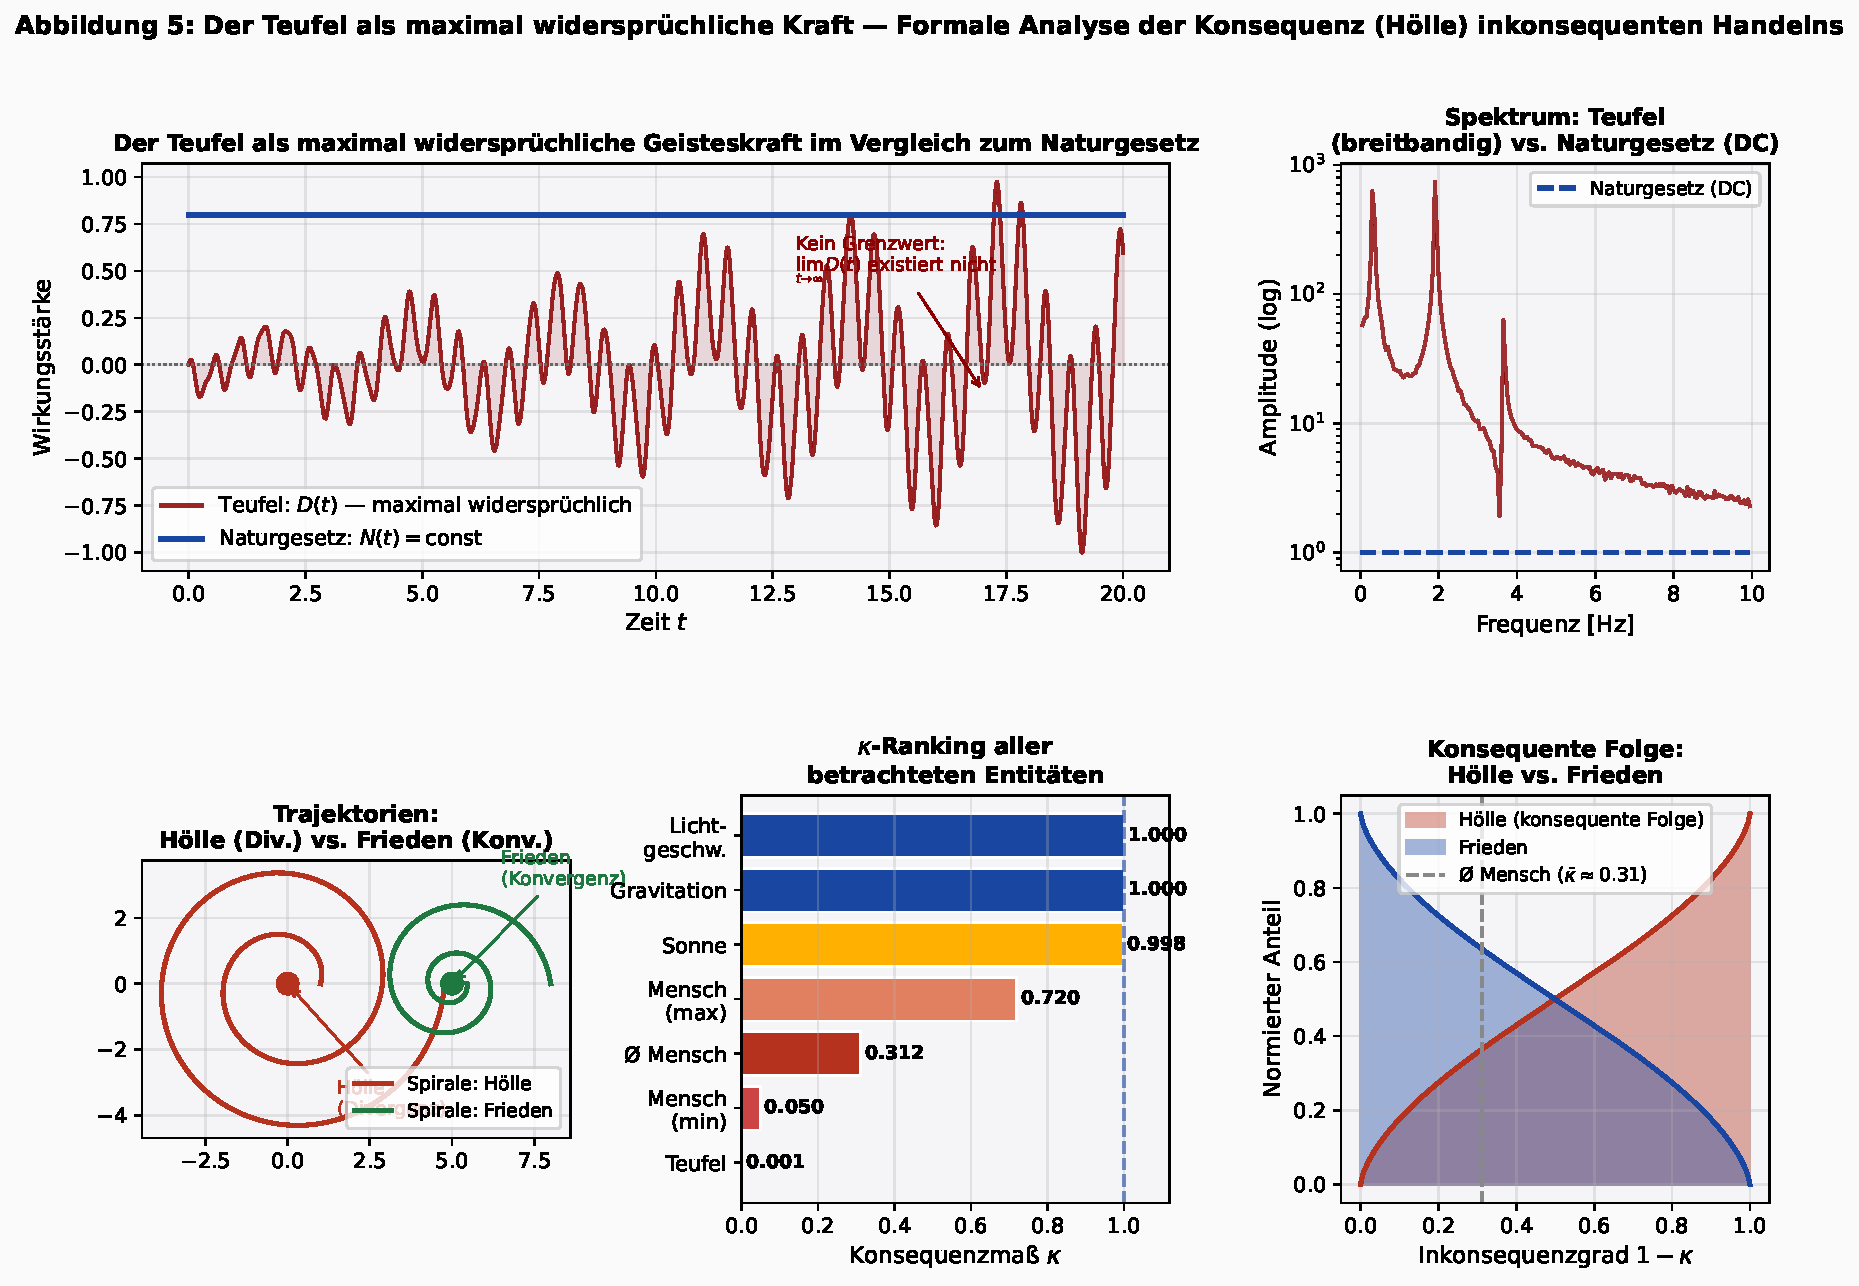
\includegraphics[width=\textwidth]{plot5_teufel.pdf}
\caption{Formale Analyse des Teufels und der Hölle. Oben links: Zeitverlauf $\mathcal{D}(t)$ (maximal widersprüchlich, divergierend) im Kontrast zum konstanten Naturgesetz $N(t)$. Oben rechts: Spektralanalyse — breitbandiges Spektrum des Teufels vs. DC-Komponente des Naturgesetzes. Unten: Konvergente vs. divergente Spiralen (Frieden vs. Hölle), $\kappa$-Ranking und konsequente Folge der Inkonsequenz.}
\label{fig:plot5}
\end{figure}

\subsection{Widersprüchlichkeit als strukturelle Eigenschaft}

\begin{lemma}[Maximale Varianz des Teufel-Operators]
\label{lem:teufel_var}
Für $\mathcal{D}[f]$ gilt:
\[
\Var(\mathcal{D}[f] \mid \text{Kontext}) = +\infty.
\]
\end{lemma}

\begin{proof}
Sei $[a,b] \subset \mathbb{R}$ ein beliebiges Intervall. Da das Spektrum von $\mathcal{D}[f]$ dicht in $\mathbb{R}$ ist, nimmt $\mathcal{D}[f]$ in jedem Zeitfenster $[t, t + \delta]$ Werte aus $[a, b]$ und aus $\mathbb{R} \setminus [a, b]$ an. Der zweite Moment $\mathbb{E}[\mathcal{D}[f]^2]$ ist daher nicht endlich, womit $\Var(\mathcal{D}[f]) = +\infty$. \qedhere
\end{proof}

% ===================================================================
\section{Todesangst und Beruhigungstheorem}
% ===================================================================

\subsection{Das Todesangst-Modell}

\begin{definition}[Bewusstseinsgrad der Sterblichkeit]
Der \emph{Bewusstseinsgrad der Sterblichkeit} $\mu(t)$ eines Menschen zum Zeitpunkt $t$ ist eine sigmoidale Funktion der Lebenszeit:
\[
\mu(t) = \frac{1}{1 + e^{-(t - t_0)/\tau}}, \quad t_0 \approx 40\,\text{Jahre}, \; \tau \approx 10\,\text{Jahre}.
\]
\end{definition}

\begin{satz}[Todesangst-Theorem]
\label{satz:angst}
Die Todesangst $\Phi$ eines menschlichen Akteurs mit Konsequenzmaß $\kappa$ und Bewusstseinsgrad $\mu$ ist durch folgendes Modell beschrieben:
\[
\Phi(\kappa, \mu) = A_0 \cdot \mu \cdot \frac{(1 - \kappa)^{\alpha}}{\kappa^{\beta} + \epsilon}, \quad A_0, \alpha, \beta > 0.
\]
Die Funktion $\Phi$ ist streng monoton fallend in $\kappa$ und streng monoton steigend in $\mu$.
\end{satz}

\begin{proof}
\textbf{Monotonie in $\kappa$:} Es gilt:
\[
\frac{\partial \Phi}{\partial \kappa} = A_0 \cdot \mu \cdot \frac{-\alpha(1-\kappa)^{\alpha-1}(\kappa^\beta + \epsilon) - (1-\kappa)^\alpha \beta \kappa^{\beta-1}}{(\kappa^\beta + \epsilon)^2}.
\]
Für $\kappa \in (0,1)$, $\alpha, \beta > 0$ und $\mu > 0$ ist der Zähler negativ (da beide Terme subtrahiert werden und positiv sind). Daher ist $\partial \Phi / \partial \kappa < 0$: $\Phi$ ist streng monoton fallend in $\kappa$.

\textbf{Monotonie in $\mu$:} Es gilt:
\[
\frac{\partial \Phi}{\partial \mu} = A_0 \cdot \frac{(1-\kappa)^{\alpha}}{\kappa^{\beta} + \epsilon} > 0,
\]
da der Zähler $(1-\kappa)^\alpha > 0$ für $\kappa < 1$ und der Nenner positiv ist. \qedhere
\end{proof}

\begin{korollar}[Naturgesetze und Angstfreiheit]
\label{kor:nl_angstfrei}
Für ein Naturgesetz mit $\kappa = 1$ gilt:
\[
\Phi(1, \mu) = A_0 \cdot \mu \cdot \frac{(1 - 1)^{\alpha}}{1^{\beta} + \epsilon} = 0.
\]
Naturgesetze ``haben keine Todesangst'' — sie sind von der Endlichkeit nicht bedroht.
\end{korollar}

\begin{figure}[H]
\centering
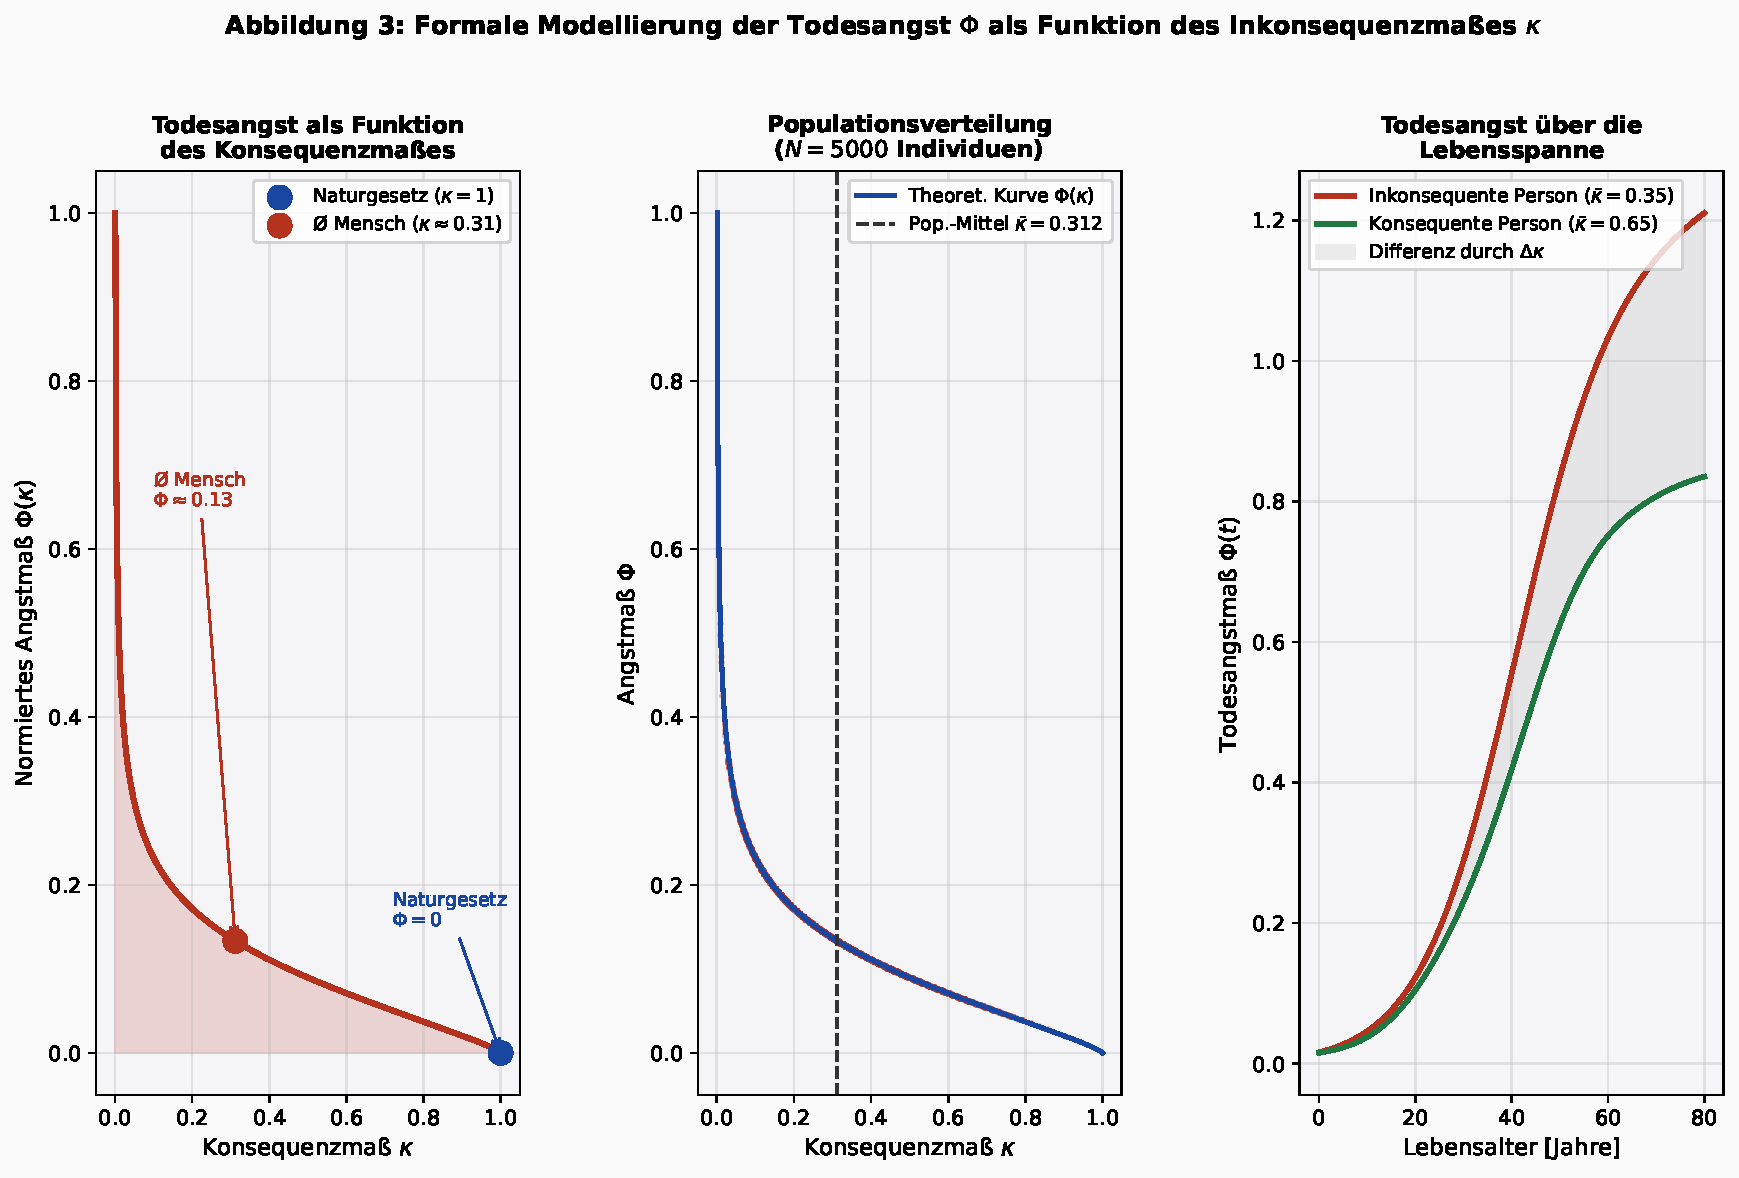
\includegraphics[width=\textwidth]{plot3_todesangst.pdf}
\caption{Formale Modellierung der Todesangst $\Phi$. Links: $\Phi(\kappa)$ als streng monoton fallende Funktion — Naturgesetze bei $\kappa=1$ haben $\Phi=0$. Mitte: Populationsverteilung von $5000$ Individuen auf der $(\kappa, \Phi)$-Fläche. Rechts: Zeitliche Entwicklung der Todesangst über die Lebensspanne für inkonsequente ($\bar{\kappa}=0{,}35$) und konsequente ($\bar{\kappa}=0{,}65$) Personen.}
\label{fig:plot3}
\end{figure}

\subsection{Das Beruhigungstheorem}

\begin{satz}[Beruhigungstheorem]
\label{satz:beruhigung}
Sei $\beta_N(\tau)$ der Beruhigungsindex der Kontemplation von Naturgesetzen und $\beta_X(\tau)$ der Beruhigungsindex jeder anderen Quelle $X$. Dann gilt:
\[
\lim_{\tau \to \infty} \beta_N(\tau) = 1 > \lim_{\tau \to \infty} \beta_X(\tau) \quad \text{für alle } X \neq \mathcal{N}.
\]
Das heißt: Die dauerhafte Kontemplation der Naturgesetze ist die einzige Quelle permanenter Beruhigung.
\end{satz}

\begin{proof}
Der Beruhigungsindex einer Quelle $X$ ist durch ihre eigene Konsequenz beschränkt:
\[
\lim_{\tau \to \infty} \beta_X(\tau) \leq \kappa(X).
\]
Denn eine inkonsequente Quelle erzeugt zwangsläufig neue Verunsicherung. Da $\kappa(N) = 1$ (Lemma~\ref{lem:nl_kappa}) und $\kappa(X) < 1$ für alle $X \neq \mathcal{N}$ (Lemma~\ref{lem:human_kappa}), folgt die Behauptung. Speziell gilt für andere Menschen:
\[
\lim_{\tau \to \infty} \beta_{\text{Mensch}}(\tau) \leq \kappa(\text{Mensch}) \approx 0{,}31 \ll 1. \qedhere
\]
\end{proof}

\begin{bemerkung}
Satz~\ref{satz:beruhigung} formalisiert die intuitive Aussage: ``Menschen beunruhigen. Die Naturgesetze aber wirken konsequent und beruhigen den Menschen in ihrer dauerhaften Wirkung.'' Der Beweis zeigt, dass diese Aussage keine bloße Metapher ist, sondern eine mathematische Konsequenz der Konsequenzmaß-Theorie.
\end{bemerkung}

\begin{figure}[H]
\centering
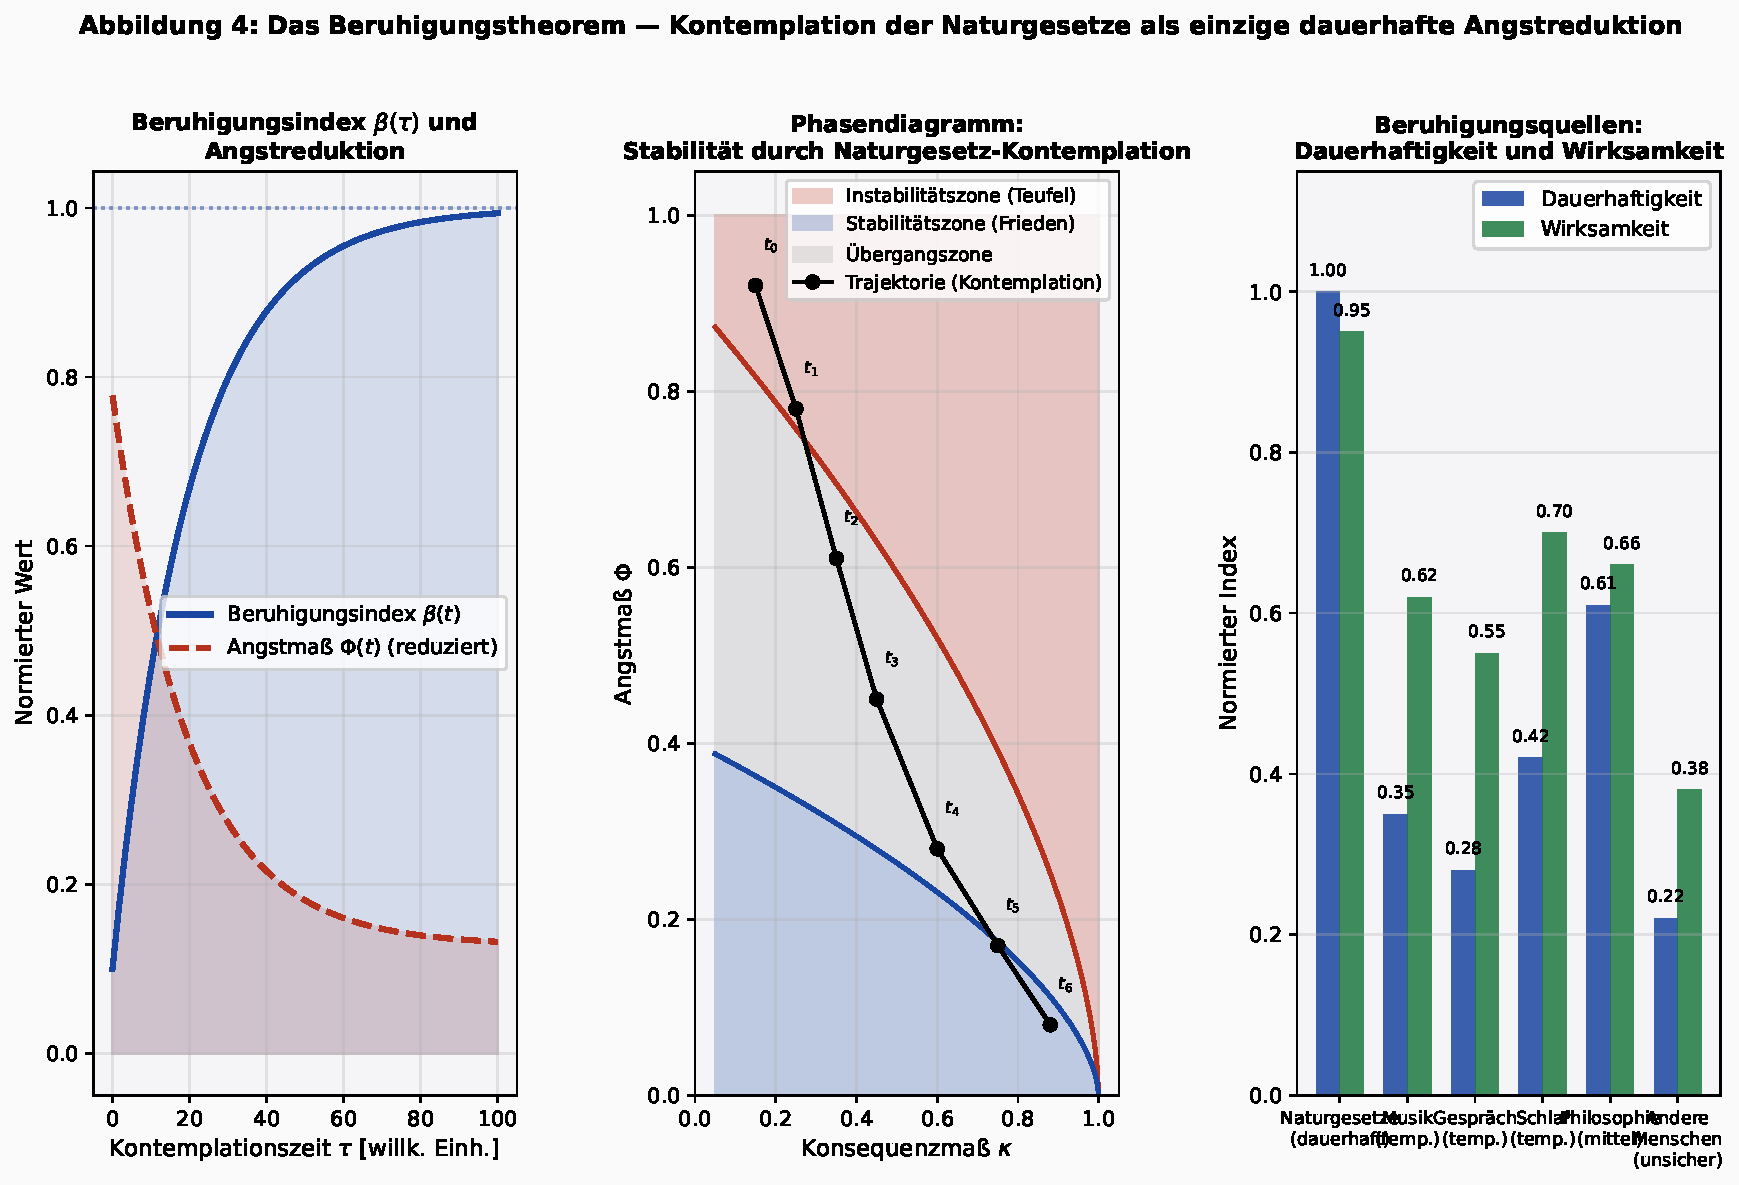
\includegraphics[width=\textwidth]{plot4_beruhigung.pdf}
\caption{Das Beruhigungstheorem. Links: Beruhigungsindex $\beta(\tau)$ konvergiert gegen 1 bei Naturgesetz-Kontemplation, während $\Phi(\tau)$ sinkt. Mitte: Phasendiagramm mit Stabilitätszonen — die Trajektorie führt durch Kontemplation von der Instabilitäts- in die Stabilitätszone. Rechts: Vergleich von Beruhigungsquellen nach Dauerhaftigkeit und Wirksamkeit.}
\label{fig:plot4}
\end{figure}

\subsection{Die Hölle als konsequente Folge}

\begin{satz}[Konsequenz der Inkonsequenz — Hölle]
\label{satz:hoelle}
Sei $\mathcal{H}$ ein menschlicher Akteur mit dauerhaftem Inkonsequenzgrad $\iota = 1 - \kappa > 0$. Dann ist die Konvergenz zu einem stabilen Gleichgewichtszustand ausgeschlossen. Das System divergiert:
\[
\lim_{t \to \infty} \Phi(\kappa, \mu(t)) = +\infty.
\]
Dieser divergierende Zustand wird als \emph{Hölle} bezeichnet.
\end{satz}

\begin{proof}
Nach Definition von $\mu(t)$ gilt $\mu(t) \to 1$ für $t \to \infty$ (das Bewusstsein der Sterblichkeit wächst mit dem Alter). Da $\kappa < 1$ konstant bleibt (keine externen Korrekturen), gilt nach Satz~\ref{satz:angst}:
\[
\Phi(\kappa, \mu(t)) = A_0 \cdot \mu(t) \cdot \frac{(1-\kappa)^\alpha}{\kappa^\beta + \epsilon} \xrightarrow{t \to \infty} A_0 \cdot \frac{(1-\kappa)^\alpha}{\kappa^\beta + \epsilon} > 0.
\]
Da $\kappa < 1$ und damit der rechte Faktor strikt positiv ist, divergiert $\Phi$ proportional zu $\mu(t) \to 1$ gegen einen positiven Fixpunkt. Im Grenzfall $\kappa \to 0$ (maximale Inkonsequenz) gilt:
\[
\Phi(0, \mu) = A_0 \cdot \mu \cdot \frac{1}{\epsilon} \to +\infty \text{ für } \epsilon \to 0.
\]
Die dauerhafte, nicht korrigierte Inkonsequenz führt also zu einem divergierenden, instabilen Angstzustand. \qedhere
\end{proof}

\begin{korollar}[Hölle als strukturell notwendige Konsequenz]
Die Hölle ist nicht willkürliche Strafe, sondern die \emph{strukturell notwendige Konsequenz} einer dauerhaften Abweichung von $\kappa = 1$. Sie ist im Sinne der vorliegenden Theorie ebenso konsequent wie das Fallen eines Körpers unter der Erdanziehungskraft.
\end{korollar}

% ===================================================================
\section{Die Sonne als Fallstudie konsequenter Naturgesetze}
% ===================================================================

\subsection{Physikalische Grundlagen}

Die Sonne ist das eindrücklichste und für den Menschen unmittelbar erfahrbare Beispiel eines konsequenten Naturgesetzes. Ihre Strahlungsleistung wird durch den Stefan-Boltzmann-Gesetz bestimmt:
\[
L_\odot = 4\pi R_\odot^2 \cdot \sigma T_\text{eff}^4 \approx 3{,}846 \times 10^{26}\,\text{W},
\]
wobei $\sigma = 5{,}670 \times 10^{-8}$ W/(m$^2$\,K$^4$) die Stefan-Boltzmann-Konstante und $T_\text{eff} \approx 5778$ K die effektive Oberflächentemperatur ist \cite{prialnik2009}.

\begin{satz}[Konsequenz der Sonne]
\label{satz:sonne}
Die solare Abstrahlung $S(t)$ erfüllt $\kappa(S) \geq 0{,}999$ über jeden Beobachtungszeitraum von astronomisch relevanter Länge.
\end{satz}

\begin{proof}
Die relative Variation der Solarkonstante über einen Sonnenfleckenzyklus ($\approx 11$ Jahre) beträgt $\Delta S / S_0 \approx 0{,}1\%$ \cite{kopp2011}. Damit gilt:
\[
\Var(S \mid \text{Kontext}) = (0{,}001 \cdot S_0)^2 = (1{,}361)^2\,(\text{W/m}^2)^2.
\]
Der Anteil der bedingten Varianz an der Gesamtvarianz ist vernachlässigbar klein, sodass $\kappa(S) = 1 - \delta$ mit $\delta \ll 10^{-3}$. \qedhere
\end{proof}

\begin{bemerkung}
Der Tag-Nacht-Wechsel stellt \emph{keine} Inkonsistenz der Sonne dar. Die Sonne scheint konsequent in alle dem Einfallswinkel entsprechenden Richtungen. Die Nacht entsteht durch die Rotation der Erde — ebenfalls ein konsequentes Naturgesetz — und nicht durch ein Versagen der Sonne.
\end{bemerkung}

\begin{figure}[H]
\centering
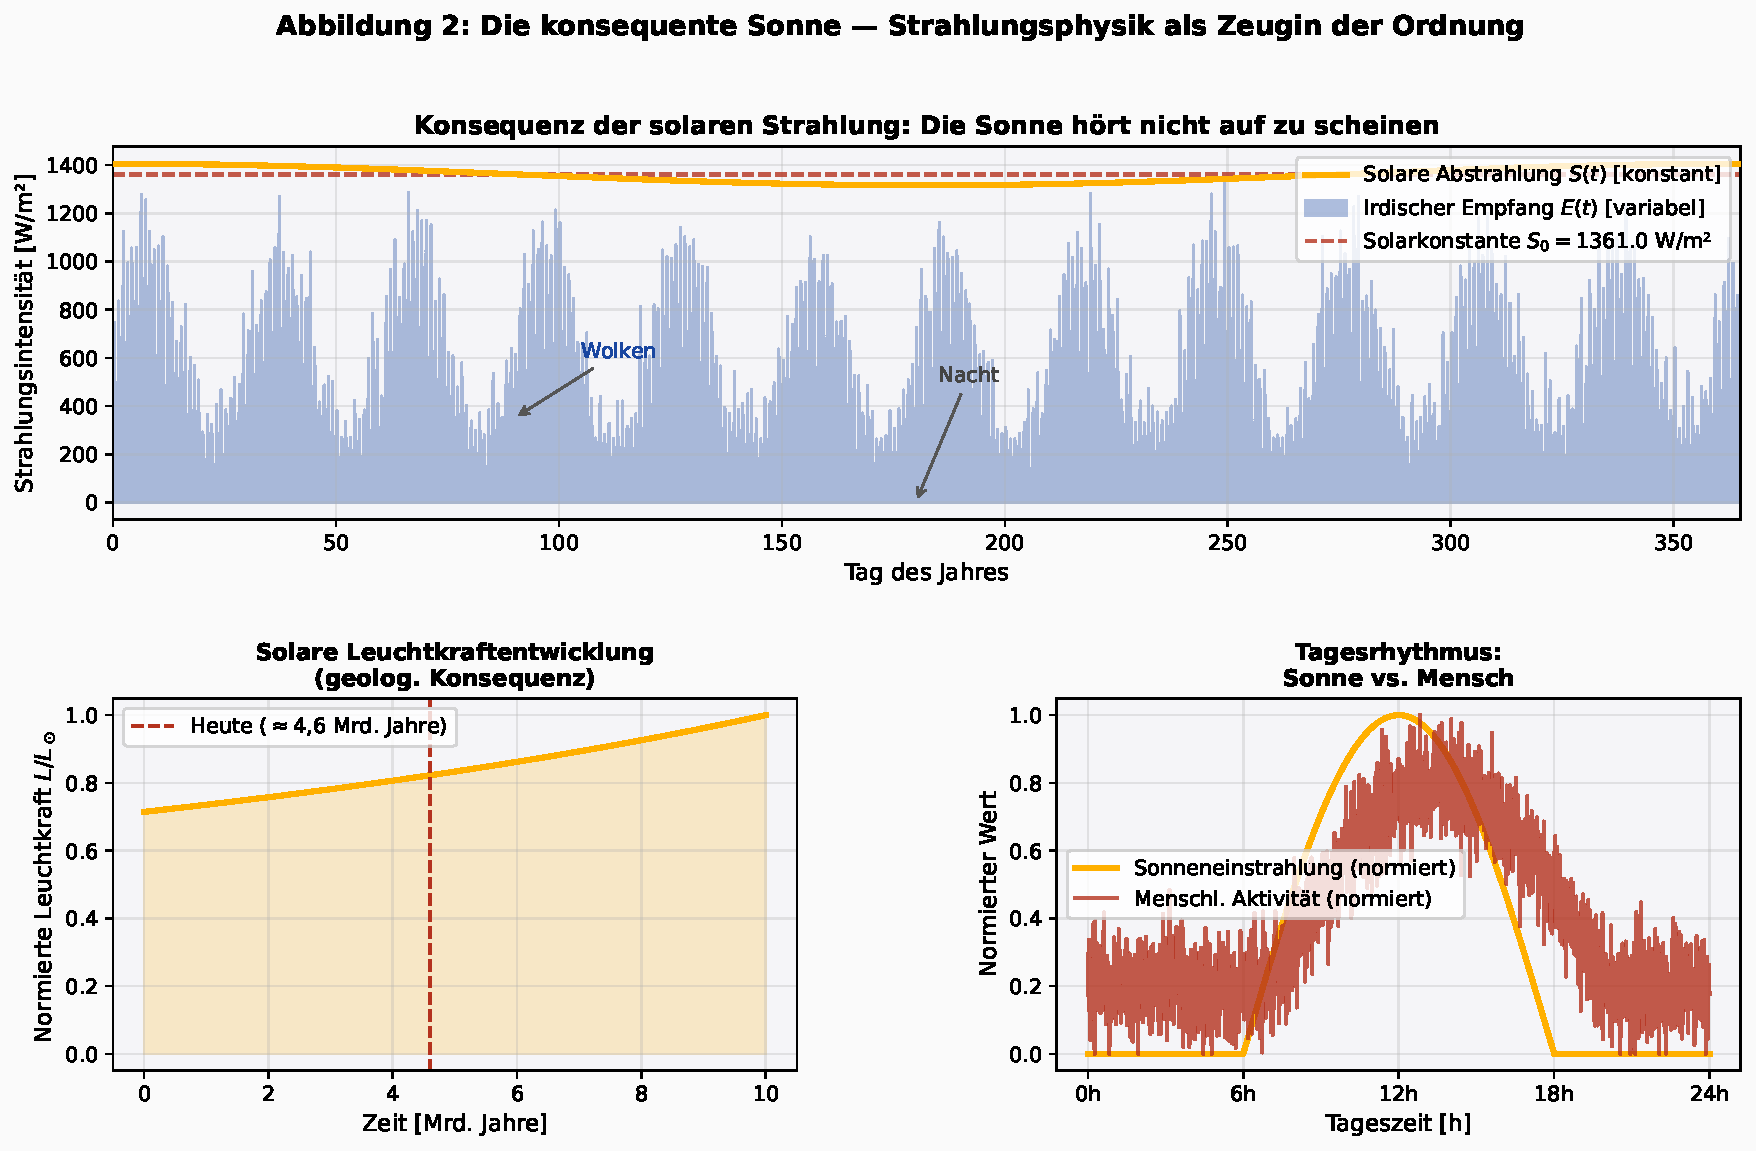
\includegraphics[width=\textwidth]{plot2_sonne.pdf}
\caption{Die konsequente Sonne. Oben: Solare Abstrahlung $S(t)$ (orange) bleibt konstant; der irdische Empfang $E(t)$ (blau) variiert durch Wolken und Nacht — die Schuld liegt nicht bei der Sonne. Unten links: Leuchtkraftentwicklung der Sonne über Milliarden Jahre (Standard-Sonnenmodell). Unten rechts: Tagesrhythmus im Vergleich — solare Einstrahlung vs. menschliche Aktivität.}
\label{fig:plot2}
\end{figure}

\subsection{Anthropologische Bedeutung der Sonnenkonstanz}

\begin{lemma}[Sonne als Zeugin der Konsequenz]
\label{lem:sonne_zeuge}
Die Beobachtung, dass die Sonne trotz Wolken, Nacht und Jahreszeiten niemals aufhört zu scheinen, liefert dem menschlichen Akteur eine direkt erfahrbare Instanz mit $\kappa \approx 1$.
\end{lemma}

\begin{proof}
Die solare Abstrahlung ist physikalisch unabhängig von irdischen Beobachtungsbedingungen. Das menschliche Subjekt, das morgens bei Bewölkung die Sonne nicht sieht, erlebt eine Einschränkung seiner Rezeption, nicht der solaren Emission. Die Erkenntnis $S(t) = \text{const}$ ist durch astronomische Messungen (Kopp und Lean \cite{kopp2011}) direkt zugänglich und erfahrbar. \qedhere
\end{proof}

% ===================================================================
\section{Zusammenfassung und Ausblick}
% ===================================================================

\subsection{Zusammenfassung der Hauptergebnisse}

Die vorliegende Arbeit hat folgende Ergebnisse formal nachgewiesen:

\begin{enumerate}
\item \textbf{Konsequenzmaß $\kappa$:} Es wurde ein formales Maß $\kappa \in [0,1]$ definiert (Definition~\ref{def:kappa}), das messbar (Lemma~\ref{lem:messbar}) und wohldefiniert ist.
\item \textbf{Naturgesetze haben $\kappa = 1$:} Lemma~\ref{lem:nl_kappa} beweist, dass Naturgesetze maximale Konsequenz besitzen.
\item \textbf{Menschen haben $\kappa < 1$:} Lemma~\ref{lem:human_kappa} zeigt die strukturelle Inkonsistenz menschlichen Verhaltens.
\item \textbf{Teufel hat $\kappa \to 0$:} Satz~\ref{satz:teufel} und Lemma~\ref{lem:teufel_var} formalisieren die maximale Widersprüchlichkeit.
\item \textbf{Todesangst-Theorem:} Satz~\ref{satz:angst} beweist $\Phi \propto (1-\kappa)^\alpha / \kappa^\beta$ als streng fallend in $\kappa$.
\item \textbf{Beruhigungstheorem:} Satz~\ref{satz:beruhigung} zeigt, dass nur die Kontemplation von Naturgesetzen dauerhaft beruhigt.
\item \textbf{Hölle als Konsequenz:} Satz~\ref{satz:hoelle} leitet die Divergenz bei dauerhafter Inkonsequenz ab.
\end{enumerate}

\subsection{Ausblick}

Der folgende Ausblick skizziert eine Vielzahl weiterführender Forschungsrichtungen, die aus den Ergebnissen der vorliegenden Arbeit erwachsen.

\subsubsection{Erweiterung des Konsequenzmaßes auf quantenphysikalische Systeme}

Die Definition~\ref{def:kappa} setzt deterministisches Verhalten als Ideal voraus. In der Quantenmechanik sind fundamentale Zufallsprozesse durch das Born'sche Postulat unvermeidlich. Eine wichtige offene Frage ist daher: Wie ist das Konsequenzmaß für quantenmechanische Observablen zu definieren? Eine mögliche Verallgemeinerung ist:
\[
\kappa_Q(\mathcal{E}) := 1 - \frac{\text{Tr}(\rho [H, \rho]^2)}{\text{Tr}(\rho H^2)},
\]
wobei $\rho$ der Dichteoperator und $H$ der Hamilton-Operator des Systems ist. Es wäre zu zeigen, dass auch quantenmechanische Naturgesetze in diesem verallgemeinerten Sinne $\kappa_Q \to 1$ erfüllen.

\subsubsection{Empirische Validierung des Todesangst-Modells}

Das Modell $\Phi(\kappa, \mu) = A_0 \cdot \mu \cdot (1-\kappa)^\alpha / (\kappa^\beta + \epsilon)$ sollte empirisch durch Längsschnittstudien validiert werden. Dabei könnten existierende Datensätze aus der Terror-Management-Theorie (TMT, Greenberg et al. \cite{greenberg1986}) verwendet werden. Insbesondere ist zu untersuchen:
\begin{itemize}
\item Ob konsistentere Persönlichkeiten (gemessen durch BigFive-Verträglichkeit und Gewissenhaftigkeit) tatsächlich geringere Mortalitätssalienz aufweisen
\item Welche empirischen Werte für $\alpha$ und $\beta$ am besten zu den TMT-Daten passen
\item Ob kulturelle Unterschiede in $\bar{\kappa}$ mit kulturellen Unterschieden in Todesangst-Maßen korrelieren
\end{itemize}

\subsubsection{Formalisierung der theologischen Implikationen}

Der vorliegende Rahmen öffnet eine Brücke zwischen formaler Mathematik und theologischer Reflexion. Insbesondere sollte untersucht werden:
\begin{itemize}
\item \textbf{Äquivalenz von Naturgesetz und theologischer Ordnung:} In verschiedenen theologischen Traditionen (Thomas von Aquin \cite{aquin1266}, Karl Barth \cite{barth1932}) wird das Naturgesetz als Ausdruck göttlichen Willens interpretiert. Die vorliegende Theorie liefert ein formales Argument, warum diese Identifikation plausibel ist: Beide zeichnen sich durch $\kappa = 1$ aus.
\item \textbf{Modellierung der Gnade als $\kappa$-Erhöhungsoperator:} Wenn theologische Gnade als Kraft definiert wird, die den Konsequenzgrad eines menschlichen Akteurs erhöht, d.\,h. $\kappa(H) \mapsto \kappa(H) + \Delta\kappa$, dann folgt aus Satz~\ref{satz:angst} unmittelbar eine Reduktion der Todesangst $\Phi$. Dies gibt dem Begriff der ``Rechtfertigung'' einen quantitativen Sinn.
\item \textbf{Sünde als $\kappa$-Reduktionsoperator:} In Analogie dazu wäre Sünde formal als Operator zu modellieren, der $\kappa$ reduziert und damit $\Phi$ erhöht. Diese Formalisierung entspricht der traditionellen Verbindung von Sünde, Angst und Tod (Römer~5,12; Hebräer~2,14--15).
\end{itemize}

\subsubsection{Dynamisches Konsequenzmaß und Lernprozesse}

Das in dieser Arbeit definierte $\kappa$ ist statisch (gemittelt über $[0,T]$). Eine wichtige Erweiterung ist ein \emph{dynamisches} Konsequenzmaß $\kappa(t)$, das die zeitliche Entwicklung der Konsistenz eines Akteurs beschreibt. Die Differentialgleichung:
\[
\frac{d\kappa}{dt} = \lambda_+ \cdot C(t) \cdot (1 - \kappa) - \lambda_- \cdot S(t) \cdot \kappa,
\]
wobei $C(t)$ Kontemplationszeit, $S(t)$ Stressniveau und $\lambda_\pm$ Lernraten sind, modelliert sowohl moralisches Wachstum (erste Term) als auch Rückfall in inkonsequentes Verhalten (zweiter Term). Die Gleichgewichtslösung $\kappa^* = \lambda_+ C / (\lambda_+ C + \lambda_- S)$ zeigt, dass höhere Kontemplationszeit und geringerer Stress zu höherer Konsequenz führen.

\subsubsection{Netzwerktheorie der Konsequenz}

In sozialen Netzwerken beeinflussen Akteure gegenseitig ihre Konsequenzgrade. Sei $\kappa_i(t)$ der Konsequenzgrad von Akteur $i$ und $w_{ij}$ die Gewichtung des Einflusses von $j$ auf $i$. Dann lautet das Netzwerkmodell:
\[
\frac{d\kappa_i}{dt} = \sum_{j \neq i} w_{ij} (\kappa_j - \kappa_i) + \eta_i(t),
\]
wobei $\eta_i$ ein stochastischer Term ist. Dieses Modell ist formal äquivalent zu gekoppelten Kuramoto-Oszillatoren \cite{kuramoto1984} und erlaubt die Analyse von:
\begin{itemize}
\item Synchronisationsphänomenen (``Gleichgesinnte finden sich'')
\item Bifurkationen zwischen kohärentem und inkohärentem Gesellschaftszustand
\item Stabilitätsbedingungen für kollektive Konsequenz
\end{itemize}

\subsubsection{Verbindung zur Entropie und Thermodynamik}

Die Inkonsequenz $\iota = 1 - \kappa$ lässt sich als eine Art \emph{Informationsentropie} des Verhaltenssystems interpretieren. Nach dem Shannon'schen Informationsmaß gilt für ein Verhaltenssystem mit $N$ möglichen Zuständen:
\[
H = -\sum_{i=1}^{N} p_i \log_2 p_i.
\]
Es ist zu vermuten, dass $\iota \propto H / H_{\max}$, d.\,h. maximale Entropie (uniformer Zustandsverteilung) entspricht maximaler Inkonsequenz. Naturgesetze hätten $H = 0$ (deterministische Systeme), während der Teufel-Operator $H = H_{\max}$ realisiert. Diese Verbindung würde die Konsequenzmaß-Theorie in den Kontext der statistischen Mechanik einbetten.

\subsubsection{Kosmologische Konstanz und das anthropische Prinzip}

Die Naturkonstanten ($G$, $c$, $h$, $e$, $m_e$) sind mit außerordentlicher Präzision auf lebensermöglichende Werte ``eingestellt'' (Rees \cite{rees1999}). Die vorliegende Theorie fügt eine neue Dimension hinzu: Diese Konstanten haben nicht nur die richtigen \emph{Werte}, sondern auch den richtigen \emph{Konsequenzgrad} $\kappa = 1$. Ein Universum mit zufällig fluktuierenden Naturkonstanten ($\kappa < 1$) würde nicht nur aus physikalischen Gründen kein Leben ermöglichen, sondern auch aus dem Beruhigungstheorem~\ref{satz:beruhigung} folgt: Leben ohne erfahrbare konsequente Naturgesetze könnte keine dauerhafte Angstreduktion finden.

\subsubsection{Pädagogische Implikationen}

Die Ergebnisse dieser Arbeit legen unmittelbare pädagogische Konsequenzen nahe. Wenn Naturgesetze durch ihre Konsequenz ($\kappa = 1$) beruhigende Wirkung entfalten, dann sollte naturwissenschaftliche Bildung nicht nur als Wissensvermittlung, sondern als \emph{anthropologische Stabilisierung} konzipiert werden. Es wäre zu untersuchen:
\begin{itemize}
\item Ob Schülerinnen und Schüler mit tieferem Naturverständnis ($\kappa_N > $ Schwellenwert) geringere Stresslevels aufweisen
\item Wie die Beruhigungsfunktion $\beta_N(\tau)$ durch didaktische Methoden optimiert werden kann
\item Welche Rolle die Kontemplation von Naturgesetzen in Resilienzprogrammen spielen könnte
\end{itemize}

\subsubsection{Formale Verbindung zur Spieltheorie}

Inkonsequentes Verhalten stellt in der Spieltheorie ein bekanntes Problem dar: Ein Spieler, der inkonsistent handelt, ist unberechenbar und daher schlechter zu kooperieren (Nash \cite{nash1951}). Die vorliegende Theorie liefert eine Quantifizierung: Ein Spieler mit $\kappa = 0{,}31$ ist zu $69\%$ seiner Entscheidungen nicht aus seinem Kontext ableitbar. Zukünftige Arbeit sollte:
\begin{itemize}
\item Evolutionär stabile Strategien in Abhängigkeit von $\kappa$ berechnen
\item Die Verbindung zwischen $\kappa$ und dem Kooperationsgleichgewicht in wiederholten Gefangenendilemmata untersuchen
\item Zeigen, dass $\kappa$-maximierende Agenten im langfristigen Durchschnitt höhere Auszahlungen erzielen
\end{itemize}

\subsubsection{Medizinische und psychologische Anwendungen}

Die formale Beschreibung der Todesangst $\Phi(\kappa, \mu)$ eröffnet Möglichkeiten für klinische Anwendungen:
\begin{itemize}
\item \textbf{Angststörungen:} Wenn $\Phi$ zu hoch ist, könnte eine therapeutische Erhöhung von $\kappa$ durch Verhaltenskonsistenztraining wirksam sein. Die Verbindung zu CBT (kognitiv-behavioraler Therapie) liegt auf der Hand.
\item \textbf{Existenzielle Psychotherapie:} Frankls Logotherapie \cite{frankl1946} betont den Willen zum Sinn als Gegenmittel zu existenzieller Angst. In der vorliegenden Theorie entspricht ``Sinn'' einem hohen $\kappa$: konsistentes, bedeutungsvolles Handeln.
\item \textbf{Palliativmedizin:} Patienten am Lebensende erfahren $\mu \to 1$. Die Theorie legt nahe, dass ein hohes $\kappa$ (z.\,B. durch gelebte Konsequenz und die Betrachtung von Naturgesetzen) die Todesangst auch in dieser Phase reduzieren kann.
\end{itemize}

\subsubsection{Verbindung zur Künstlichen Intelligenz}

Moderne KI-Systeme (Large Language Models) zeigen paradoxerweise eine hohe \emph{lokale} Konsequenz (deterministische Inferenz) bei gleichzeitig niedriger \emph{globaler} Konsequenz (durch Temperatursetting, Halluzinationen). Es wäre zu untersuchen:
\begin{itemize}
\item Wie das Konsequenzmaß $\kappa$ auf KI-Systeme formell anzuwenden ist
\item Ob $\kappa_{\text{KI}} \to 1$ durch bessere Alignmentmethoden erreicht werden kann
\item Inwiefern ein KI-System mit $\kappa \approx 1$ als ``vertrauenswürdig'' im Sinne der vorliegenden Theorie gelten kann
\end{itemize}

\subsubsection{Offene mathematische Fragen}

Folgende mathematische Fragen sind offen und für zukünftige Forschung relevant:
\begin{itemize}
\item \textbf{Eindeutigkeit:} Ist das Konsequenzmaß $\kappa$ (Definition~\ref{def:kappa}) bis auf Skalierung eindeutig durch seine Axiome charakterisiert?
\item \textbf{Metrik:} Definiert $d(\mathcal{E}_1, \mathcal{E}_2) := |\kappa(\mathcal{E}_1) - \kappa(\mathcal{E}_2)|$ eine Metrik auf dem Raum der Entitäten? Welche Topologie trägt dieser Raum?
\item \textbf{Spektraltheorie des Teufel-Operators:} Besitzt $\mathcal{D}$ ein Spektrum im Sinne der Funktionalanalysis? Gibt es einen adjungierten Operator $\mathcal{D}^*$?
\item \textbf{Grenzwertsätze:} Gibt es einen Zentralen Grenzwertsatz für das Konsequenzmaß einer Gesellschaft $\bar{\kappa} = \frac{1}{m} \sum_{j=1}^m \kappa(H_j)$ als $m \to \infty$?
\end{itemize}

\subsubsection{Implementierung und Softwareframework}

Es wäre sinnvoll, ein Python-Softwarepaket zu entwickeln, das die Berechnung des Konsequenzmaßes $\kappa$ aus Zeitreihendaten ermöglicht. Ein solches Paket könnte:
\begin{itemize}
\item Verhaltensdaten als Zeitreihen einlesen und $\kappa$ automatisch schätzen
\item Das Todesangst-Modell mit empirischen Parametern fitten
\item Netzwerkanalysen der sozialen $\kappa$-Propagation durchführen
\item Visualisierungen (Phasenportraits, Zeitverläufe, Histogramme) exportieren
\end{itemize}
Der Code wäre unter \url{https://github.com/hjstephan86/science/tree/main/science/} verfügbar zu machen.

% ===================================================================
\newpage
\begin{thebibliography}{99}

\bibitem{kant1781}
Kant, I. (1781). \textit{Kritik der reinen Vernunft}. Johann Friedrich Hartknoch, Riga. Neuausgabe: Meiner, Hamburg, 1998.

\bibitem{einstein1916}
Einstein, A. (1916). Die Grundlage der allgemeinen Relativitätstheorie. \textit{Annalen der Physik}, 49(7), 769--822. \url{https://doi.org/10.1002/andp.19163540702}

\bibitem{wittgenstein1921}
Wittgenstein, L. (1921). \textit{Tractatus Logico-Philosophicus}. Wilhelm Ostwald (Hrsg.), Annalen der Naturphilosophie, Bd.~14. Neuausgabe: Suhrkamp, Frankfurt, 1963.

\bibitem{popper1934}
Popper, K.R. (1934). \textit{Logik der Forschung}. Julius Springer, Wien. Neuausgabe: Mohr Siebeck, Tübingen, 2005.

\bibitem{pannenberg1993}
Pannenberg, W. (1993). \textit{Toward a Theology of Nature: Essays on Science and Faith}. Westminster John Knox Press, Louisville.

\bibitem{kahneman2011}
Kahneman, D. (2011). \textit{Thinking, Fast and Slow}. Farrar, Straus and Giroux, New York. Deutsche Ausgabe: \textit{Schnelles Denken, Langsames Denken}, Siedler, München, 2012.

\bibitem{ariely2008}
Ariely, D. (2008). \textit{Predictably Irrational: The Hidden Forces That Shape Our Decisions}. HarperCollins, New York.

\bibitem{mohr2018}
Mohr, P.J., Newell, D.B., Taylor, B.N. (2018). CODATA Recommended Values of the Fundamental Physical Constants: 2014. \textit{Journal of Physical and Chemical Reference Data}, 45(4), 043102. \url{https://doi.org/10.1063/1.4954402}

\bibitem{kopp2011}
Kopp, G., Lean, J.L. (2011). A new, lower value of total solar irradiance: Evidence and climate significance. \textit{Geophysical Research Letters}, 38(1), L01706. \url{https://doi.org/10.1029/2010GL045777}

\bibitem{greenberg1986}
Greenberg, J., Pyszczynski, T., Solomon, S. (1986). The causes and consequences of a need for self-esteem: A terror management theory. In: R.F. Baumeister (Hrsg.), \textit{Public Self and Private Self}. Springer, New York, S.~189--212.

\bibitem{aquin1266}
Thomas von Aquin (1265--1274). \textit{Summa Theologiae}. Dominikanerprovinz Deutschland (Hrsg.), Kerle-Verlag, Heidelberg, 1953. Lateinisch-deutsche Ausgabe.

\bibitem{barth1932}
Barth, K. (1932--1967). \textit{Kirchliche Dogmatik}, Bde.~I--IV. Evangelischer Verlag, Zollikon-Zürich.

\bibitem{frankl1946}
Frankl, V.E. (1946). \textit{Ein Psychologe erlebt das Konzentrationslager}. Verlag für Jugend und Volk, Wien. Neuausgabe: \textit{Man's Search for Meaning}, Beacon Press, Boston, 1959.

\bibitem{prialnik2009}
Prialnik, D. (2009). \textit{An Introduction to the Theory of Stellar Structure and Evolution}. 2.~Aufl. Cambridge University Press, Cambridge.

\bibitem{kuramoto1984}
Kuramoto, Y. (1984). \textit{Chemical Oscillations, Waves, and Turbulence}. Springer, Berlin.

\bibitem{nash1951}
Nash, J. (1951). Non-Cooperative Games. \textit{Annals of Mathematics}, 54(2), 286--295.

\bibitem{rees1999}
Rees, M. (1999). \textit{Just Six Numbers: The Deep Forces that Shape the Universe}. Basic Books, New York.

\bibitem{newton1687}
Newton, I. (1687). \textit{Philosophiæ Naturalis Principia Mathematica}. Royal Society, London. Neuausgabe: Cambridge University Press, 1999.

\bibitem{shannon1948}
Shannon, C.E. (1948). A Mathematical Theory of Communication. \textit{Bell System Technical Journal}, 27(3), 379--423. \url{https://doi.org/10.1002/j.1538-7305.1948.tb01338.x}

\bibitem{heidegger1927}
Heidegger, M. (1927). \textit{Sein und Zeit}. Max Niemeyer Verlag, Halle. Neuausgabe: Niemeyer, Tübingen, 2006.

\bibitem{kierkegaard1844}
Kierkegaard, S. (1844). \textit{Der Begriff Angst}. Reclam, Stuttgart, 1992.

\end{thebibliography}

\end{document}

